\documentclass[11pt,a4paper]{article}
\usepackage[ngerman]{babel}
\usepackage[TS1,T1]{fontenc}
\usepackage[utf8x]{inputenc}
\selectlanguage{ngerman}
\usepackage{theorem}
\usepackage[scaled=0.9]{helvet}
\usepackage{amsmath}
\usepackage{amssymb}
\usepackage{hyperref}
\usepackage{stmaryrd}
\usepackage{pgf,tikz}
\usepackage{relsize}
\usepackage{enumitem}
\usepackage{graphicx}
\usepackage{algpseudocode,amsmath,xifthen}

\newcounter{numb}
\theoremstyle{break}
\theorembodyfont{\upshape}
   	\newtheorem{exercise}{Exercise}[numb]
\setlength{\oddsidemargin}{0cm}
\setlength{\textwidth}{16cm}
\setlength{\textheight}{23cm}
\setlength{\topmargin}{-2cm}

\usetikzlibrary{shapes,arrows,automata,positioning,decorations.fractals}
\renewcommand\familydefault{\sfdefault}

\newcommand{\header}[2]{
\begin{minipage}[b]{\textwidth}
		\parbox[t]{5cm}{%
			
\includegraphics[width=4cm]{unilogo}
			\hfill
		}
		\parbox[b]{11cm}{%
			%\scshape%
			Heinrich-Heine-University D\"usseldorf\\
			Computer Science Department\\
			Software Engineering and Programming Languages\\
			%Professor Dr.\ M.\ Leuschel
		Philipp K\"orner
}
		
\end{minipage}
	\begin{center}
		\bf
		Functional Programming -- WT 2024 / 2025\\
        Reading Guide {\thenumb}: {#1}
	\end{center}

    \pagestyle{empty}
    \paragraph{Timeline:} This unit should be completed by {#2}.
}

\usepackage{multicol}
\setcounter{numb}{5}


\begin{document}

\begin{minipage}[b]{\textwidth}
	\parbox[t]{5cm}{%
		
\includegraphics[width=4cm]{unilogo}
		\hfill
	}
	\parbox[b]{11cm}{%
		%\scshape%
		Heinrich-Heine-University D\"usseldorf\\
		Computer Science Department\\
		Software Engineering and Programming Languages\\
		%Professor Dr.\ M.\ Leuschel
		Philipp K\"orner
	}
\end{minipage}
\begin{center}
	\bf
	Functional Programming -- WISE 2020 / 2021\\
	Reading Guide 5: Simplicity
\end{center}

\pagestyle{empty}

\paragraph{Deadline:} This unit should be completed by 10.12.2020.

\section{Material} 

\begin{itemize}
\item Rich Hickey: Simple Made Easy \url{https://www.infoq.com/presentations/Simple-Made-Easy/}
\item Rich Hickey: Simplicity Matters \url{https://www.youtube.com/watch?v=rI8tNMsozo0} (22:02 -- 33:36)
\item Stuart Halloway: Simplicity Ain't Easy \url{https://www.youtube.com/watch?v=cidchWg74Y4}
\item Ben Moseley, Peter Marks: Out of the Tar Pit \url{https://github.com/papers-we-love/papers-we-love/blob/master/design/out-of-the-tar-pit.pdf} (Sections 1 -- 7)\footnote{The relevant part of the article is relatively long, but easy to read.}
\item The Joy of Clojure, chapter 14
\end{itemize}


\section{Learning Outcomes}

After completing this unit you should be able to

\begin{itemize}
    \item explain and differentiate the terms simple, easy, hard and complex.
    \item recognize complexity.
    \item describe approaches that can be used to understand programs.
    \item name and identify causes of complexity.
    \item describe the influence of state.
    \item describe the differences in the approaches to complexity in functional and object-oriented programming.
    \item identify and differentiate essential and non-essential types of complexity.
\end{itemize}



\section{Exercises}

\begin{exercise}[Fixed point algorithm]

Reading Guide 03 asked you to implement Newton's method.
This exercise is about abstracting the solution to a general fixed point method.
Newton's method is then a special case of this abstraction.
Proceed as follows:
    
\begin{enumerate}[label=\alph*)]
\item Write a function \texttt{(defn fixedpoint [F guess eps?] ...)}, which computes a fixed point of $F$ from an initial value $guess$.
    The accuracy $eps?$ should itself be a function that receives two inputs: (the new and old value) and returns true if the two values match sufficiently well.

    You can use the following code (or your own solution) as a basis:

\begin{verbatim}
(defn newton [f f']
  (fn newton-fn [x eps]
    (let [next-x (- x (/ (f x)
                         (f' x)))]
      (if (< (abs (- next-x x)) eps)
        next-x
        (newton-fn next-x eps)))))
\end{verbatim}

\item Write Newton's method as instance of this fixed point function.
\item Which aspects of the implementation of Newton's method have you abstracted and decomplected here?
\end{enumerate}
\end{exercise}

\begin{exercise}[Graph]
The following exercise asks you to implement different functions operating on a graph. As representation of the graph we use a map.

\begin{multicols}{2}[]
\begin{verbatim}
(def g {:nodes #{:a :c :b :d :e}, 
        :edges #{[:b :c] [:e :e] 
                 [:c :e] [:a :d] 
                 [:a :e] [:d :b] 
                 [:b :a]}})
\end{verbatim}

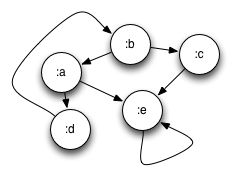
\includegraphics[width=5cm]{graph}

\end{multicols}



\begin{enumerate}[label=\alph*)]
  \item Write a function \texttt{(defn dom [g] ...)}, which returns a subset of nodes that have an outgoing edge.
  %(defn dom [g] (into #{} (map first (:edges g))))
  \item Write a function \texttt{(defn ran [g] ...)}, which returns a subset of nodes that have an incoming edge.
  %(defn ran [g] (into #{} (map second (:edges g))))
  \item Implement a function \texttt{(defn tc [g] ...)}, which takes a graph as a parameter and returns a graph describing the transitive closure of the input. {\it Note: Consider whether you can use the fixed point function or a generalized version of a fixed point function to do this.}
  
  \item Implement the function \texttt{(defn trc [g] ...)}, which computes the transitive, reflexive closure.

  \item Write a predicate \texttt{(defn path? [g start end] ...)}, that returns a truthy value if Graph $g$ contains a path from $start$ to $end$ or a falsey value if there is no such path. Make sure that your predicate also terminates if the graph is cyclic.
\end{enumerate}
\end{exercise}


\section*{Questions}
If you have any questions, please contact Philipp K"orner (\texttt{p.koerner@hhu.de}).
\end{document}

